\hypertarget{apr__ldap__rebind_8h}{}\section{/usr/local/src/github/\+Codebase/httpd-\/2.4.29/srclib/apr-\/util/include/apr\+\_\+ldap\+\_\+rebind.h File Reference}
\label{apr__ldap__rebind_8h}\index{/usr/local/src/github/\+Codebase/httpd-\/2.\+4.\+29/srclib/apr-\/util/include/apr\+\_\+ldap\+\_\+rebind.\+h@{/usr/local/src/github/\+Codebase/httpd-\/2.\+4.\+29/srclib/apr-\/util/include/apr\+\_\+ldap\+\_\+rebind.\+h}}


\hyperlink{namespaceApache}{Apache} L\+D\+AP library.  


This graph shows which files directly or indirectly include this file\+:
\nopagebreak
\begin{figure}[H]
\begin{center}
\leavevmode
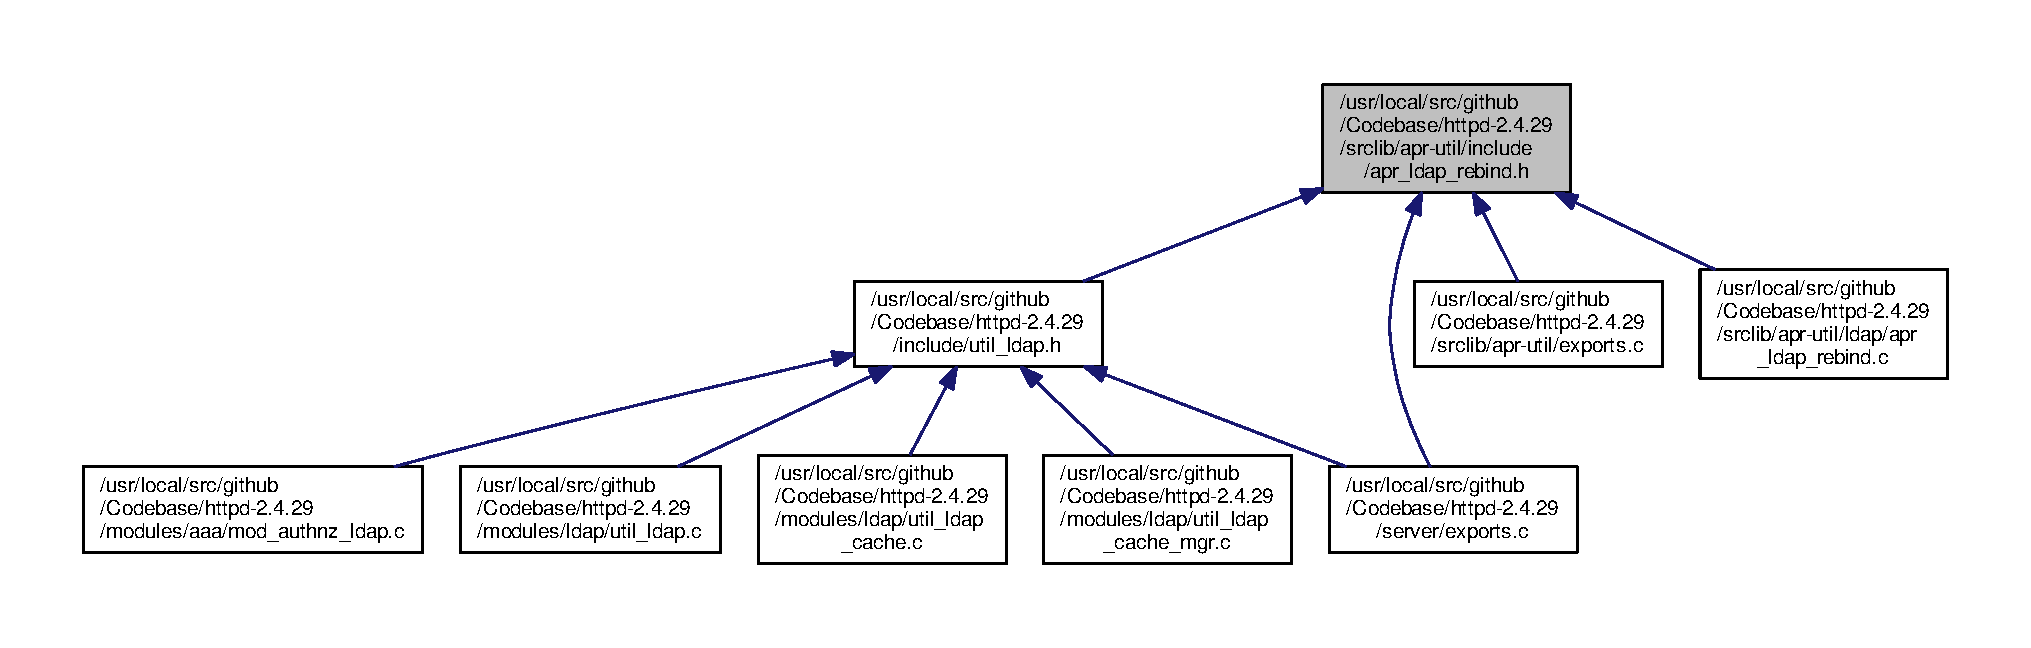
\includegraphics[width=350pt]{apr__ldap__rebind_8h__dep__incl}
\end{center}
\end{figure}


\subsection{Detailed Description}
\hyperlink{namespaceApache}{Apache} L\+D\+AP library. 

The A\+PR L\+D\+AP rebind functions provide an implementation of a rebind procedure that can be used to allow clients to chase referrals, using the same credentials used to log in originally.

Use of this implementation is optional. 